\documentclass[10pt,a4paper]{scrreprt}
\usepackage[utf8]{inputenc}
\usepackage[english]{babel}
\usepackage{amsmath}
\usepackage{amsfonts}
\usepackage{amssymb}
\usepackage{pgfplots}
\usepackage{caption}
\usepackage{graphicx}
\usepackage{tikz-3dplot}
\usepackage{subcaption}
\usepackage{float}
\usepackage{multirow,rotating}
\usepackage[autostyle]{csquotes}

\usepackage[backend=biber,style=authoryear-comp]{biblatex}
\addbibresource{Meine Bibliothek.bib}


\begin{document}
\chapter{Introduction}
The definition of the relevant market is a basic prerequisite for any political decisions about possible market interventions. It is a competition policy concept with the aim to identify the competitive environment within an industry (\cite{argentesi_market_2005}). In case of a wrong understanding of the relevant market, regulatory interference might worsen the market situation, if for instance an antitrust authority imposes a socially inefficient regulation on an incumbent that in fact faces sufficient competition or blocks a welfare-enhancing merger. The objective of market definition is to search for the smallest set of products competing between them in order to guide the antitrust investigation. It therefore analyzes substitutional relationships between products or product groups to identify competitive constrains faced by a firm or a group of firms. If consumers can easily switch between two products, a firm will be constrained regarding the ability to raise prices (\cite{filistrucchi_market_2013}).

The reasoning of demand substitution is implemented in the conceptual tool of the so-called SSNIP (Small but Significant Non-transitory Increase in Price) test. According to this test, the narrowest market is defined as a set of products for which a hypothetical monopolist could sustainably raise prices above the current level by a given amount (usually 5\%-10\%) without losing demand. Following the European Commission "[…] differences in product characteristics are not in themselves sufficient to exclude demand substitutability […]” (\cite{european_commission_commission_1997}), which makes it necessary to define a market applying analytical tools like the SSNIP test. However, as we will explain below, in the context of two-sided markets\footnote{Two-sided markets are a special case of multi-sided markets, or platform markets. For simplicity, we will refer to two-sided markets, even though most of our argumentation is true for multi-sided markets.} this test needs further adaptations.

Two-sided markets are characterized by intermediaries or platforms that sell two different products to two different groups of agents.  These two groups are interconnected as they mutually influence each other’s demand. The platforms recognize the interconnection and choose the price structure according to the relative size of the indirect network effects. In a more restrictive definition of two-sided markets, \cite{rochet_platform_2003} determine those markets as two-sided, if the price structure is non-neutral, i.e., the volume of transactions and the participation levels vary as the price structure varies, holding the price level constant. This definition stresses the importance of the distinction between the price level, which is the sum of the prices charged by a platform on both sides, and price structure, which is the allocation of the price level among the two sides. Traditional antitrust instruments like the SSNIP test are designed for single-sided markets, using the price level to analyze a market. Drawing from the economic literature on market definition with interdependencies in demand, it can be shown that tese instruments cannot be easily applied in case of two-sided platform competition (\cite{noel_analyzing_2005} \cite{filistrucchi_market_2013}).

Although two-sided markets are not invented by the digital revolution, digital markets very often demonstrate a market structure with two or more consumer-groups that are related via indirect network effects and are connected by platforms. A very prominent example can be found within the search engine market, where Google connects at least two market-sides: the demand for search query and the demand for placing advertisement. It can easily be seen, that advertisers value a big group on the other market side, as their scope and therefore the effectiveness of advertisement grows. The value of the search query on the other market side might be influenced negatively or positively by the amount of advertisement. This indirect network effect pretty much depends on the quality of the advertisement and on the consumers demand on personalized advertisement.

Two-sided markets can also be found within more traditional markets like credit cards, newspaper or shopping mall. These markets play an important role when analyzing the nature of two-sided markets as they offer an explicit market structure and available data. Requirements that cannot easily be found within digital markets due to rapidly changing market dynamics. Nevertheless, the rapid growth of digital markets calls for an analytical tool that can be applied to define the relevant market.

Based on economic reasoning we will explain why the application of a SSNIP test - being the most important analytical tool for regulatory and antitrust cases in the EU - on a two-sided market leads to a mistakenly market definition. Furthermore we present an approach to analyze market structure by looking at the cross correlations of quantities of potential competitors. As a benchmark for the cross correlation coefficients we will simulate a Cournot duopol model. 

The paper proceeds as follows: chapter \ref{litrev} presents a review of the relevant literature on market definition and two-sided markets; chapter \ref{SSNIP} analyses the consequences of applying a SSNIP test for market definition on two-sided markets; chapter \ref{model} presents a Cournot duopol model of platform competition and the results of a Monte Carlo simulation for this model; chapter \ref{empirical}  explains how we use empirical data to test our approach of market definition using cross-correlation functions of quantities in media markets.  


\chapter{Literature Review}\label{litrev}
This paper is related to a relatively recent line of economic literature, investigating the implications of two-sided markets on competition policy and offering different approaches to deal with the feedback effects between demand on multiple market sides. While the first policy contributions mainly criticized the application of standard policy to those markets (\cite{wright_one-sided_2004}; \cite{leonello_horizontal_2010}; \cite{chandra_mergers_2009}), more recent work has also intended to suggest alternative approaches (\cite{argentesi_estimating_2007}; \cite{song_estimating_2015}). We try to contribute to the latter by offering a new approach to define a two-sided market. 

The literature of two-sided markets was pioneered by the theoretical work of \cite{caillaud_chicken_2003}, \cite{rochet_platform_2003}, \cite{evans_antitrust_2003} and \cite{armstrong_competition_2006}, whereby the definition given by \cite{evans_antitrust_2003} can be seen as a particular case of the more general definition proposed by \cite{rochet_platform_2003} (\cite{filistrucchi_identifying_2012}). \cite{rochet_platform_2003} as well as \cite{armstrong_competition_2006} both provide a theoretical concept to analyze how platforms chose prices in a market with two consumer sides (networks) showing indirect network effects. However, there are a number of modeling differences between the two articles with regard to (a) the platform's cost structure, (b) the fee the consumers on both market sides have to pay and (c) the source of consumer heterogeneity. For most of their analysis \cite{rochet_platform_2003} assume that the platform incurs in a per-transaction cost and charges a usage fee, whereas \cite{armstrong_competition_2006} considers membership fees and per-agent cost.\footnote{\cite{rochet_platform_2003} as well as \cite{armstrong_competition_2006} both consider the case where there are fixed fees as well as per-transaction fees for model where consumers can only single-home.} With respect to the source of consumer heterogeneity (c) in \cite{rochet_platform_2003} consumers are heterogenous in the benefit they get from the interaction with the respective other market side or, in other words, the indirect network effect varies between the consumers. In \cite{armstrong_competition_2006} the indirect network effect only differs between the market side and is homogenous among agents on the same side. Heterogeneity is given by differences in consumers' membership values.\footnote{A more detailed discussion of these assumptions with regard to our approach is provided in \ref{model}} For the monopoly case the equilibrium prices of a profit-maximizing platform on one market side is given by the cost of providing the service, adjusted downwards by the magnitude of the indirect network effect and adjusted upwards by the elasticity of demand on that side (\cite{armstrong_competition_2006}). In the model of \cite{rochet_platform_2003} the price level charged by a profit-maximizing platform will be given the classical Lerner formula, where elasticity is the sum of the two elasticities in each side.  
 
In a more recent paper \cite{rochet_two-sided_2006} provide an analysis of the monopoly case, where agents' are heterogeneous both regarding the indirect network effect and the membership value. However, \cite{weyl_price_2010} generalizes the model in \cite{rochet_two-sided_2006} as he allows agents to be heterogenous in the type of the indirect network effects: The membership externality, occurring when an additional membership has a positive effect on the other market side, and usage externality, when the benefit is originated by an additional transaction. To avoid the equilibrium multiplicity and to overcome the coordination problem that maybe faced by a platform in having both sides "on board",\footnote{This coordination problem is also known as chicken $\&$ egg problem (\cite{caillaud_chicken_2003})} \cite{weyl_price_2010} assumes, that the platform directly choses the participation level on both sides, rather then the price structure.\footnote{He refers to this as insulated tariffs (See also \cite{white_insulated_2012})}

To identify a market as being two-sided, the interconnection of the two market sides has to be detected. Most of the literature related to the quantification of the indirect network effects have based their analysis on electronic payments system industries (\cite{ackerberg_quantifying_2006}; \cite{rysman_empirical_2007}) or magazine and newspaper industries (\cite{kaiser_price_2006}, \cite{argentesi_estimating_2007}). \cite{rysman_competition_2004} estimates a structural model of two-sided markets to measure indirect network effects in the market for Yellow Pages. In his setting the platform maximizes profits in choosing the price only on the advertiser side, as reader get the service for free. In \cite{argentesi_estimating_2007}, instead publishers’ profits are the sum of advertising profits and profits from circulation. They use data on the Italian newspaper industry to offer an alternative approach to test for collusion using a structural econometric model characterized by only one indirect network effect from reader to advertiser. \cite{argentesi_market_2005} provide a generalized framework of \cite{argentesi_estimating_2007} with indirect network effects on both market sides (See also \cite{filistrucchi_merger_2010}). Whereas no effect of advertising on the number of readers was found in the daily newspaper market in the US (\cite{fan_ownership_2013}) and in the Belgian daily newspaper market (\cite{cayseele_prices_2009}), \cite{kaiser_price_2006} find that advertising increases readers demand for magazines in Germany. They use an adopted version of the model proposed in \cite{armstrong_competition_2006}. However, \cite{wilbur_two-sided_2008} found a negative effect of advertising on viewers in the television market. His main conclusions are that viewers tend to be adverse to advertising, that advertiser preferences influence network choices more strongly than viewer preferences, and that advertisement avoidance tends to increase equilibrium advertising quantities and decrease network revenues.

As mentioned above, earlier policy contributions criticize the application of standard competition policy on markets that exhibit at least one indirect network effect. \cite{evans_antitrust_2003}, \cite{evans_industrial_2007} \cite{wright_one-sided_2004} and \cite{kaiser_price_2006} are prominent examples of papers that have focused on competition policy on two-sided markets. They have pointed out that in the presence of indirect network externalities the efficient price structure does not reflect the ratio of marginal cost, nor does increased competition necessarily leads to a more efficient market outcome or merger leads to increased prices.\footnote{\cite{malam_mergers_2011} uses an oligopoly model of competition with differentiated products (based on the approach of \cite{salop_monopolistic_1979}) where ad-sponsored media platforms charge a zero price to viewers when competing simultaneously for advertisers. He shows, that mergers among ad-sponsored platforms have a competition-intensifying effect, which offsets the incentive to increase prices on the advertiser side.} They show that relying on conventional methods to analyze mergers in two-sided markets will lead to significantly different results than using methods that explicitly incorporate the two-sided nature of this markets. \cite{evans_antitrust_2003} argues, that defining a relevant market for antitrust purposes looking at only one side can lead to a market definition which is too narrow. In a more recent study \cite{evans_analysis_2008} analyze the Google and DoubleClick case, confirming, that the Lerner pricing formula does not hold for two-sided markets. While predatory pricing is a practice that harms competition in case of traditional industries\footnote{Industries with only one market side.}, selling a product below marginal cost\footnote{Or even for free, as is the case for the search-engine market as well as many digital markets.} can be a profit maximizing strategy rather than an attempt to predate in a two-sided market (\cite{wright_one-sided_2004}). \cite{wright_one-sided_2004} also argues, that increased competition does not necessarily lead to more efficient prices from the social point of view. A analysis of the Canadian newspaper industry shows, that mergers in two-sided markets may not necessarily lead to higher prices for either side of the market. Even a merger to monopoly might raise welfare and do so even in the absence of efficiency gains (\cite{leonello_horizontal_2010}). These papers emphasizes  the need for alternative approaches to adopt competition policy that adequately hits the requirements of two-sided markets. 

\cite{filistrucchi_ssnip_2008} discuses the application of a modified SSNIP test in order to determine the relevant two-sided market. He suggests a distinction of the two-sided markets regarding the observability of transaction costs.\footnote{Whereas \cite{filistrucchi_ssnip_2008} uses the terms “media type” and “payment card type”, \cite{filistrucchi_market_2013} use the terms “non-transaction” and “transaction” marktes.} In the "payment card type" market the platform can observe the transaction cost between the two market sides, whereas in the "media type" market the transaction cost does not exist (or is not observable to the platform, e.g. reader reads an ad). In \cite{filistrucchi_market_2013} the authors point out, that in two-sided non transaction markets, two (interrelated) markets need to be defined, while in transaction markets, only one market side should be defined.\footnote{We will discuss this suggestion as well as the application of a modified SSNIP test in the upcoming chapter \ref{SSNIP}.} \cite{emch_market_2006} and \cite{alexandrov_antitrust_2011} show how a SSNIP test should be performed in a two-sided non transaction market. \cite{white_insulated_2012} present a UPP formulae for two-sided markets assuming that firms charge insulating tariffs, meaning that platforms choose quantities and then support those quantities by the corresponding insulating tariffs and \cite{noel_analyzing_2005} suggests an extension of the Critical Loss Analysis as an alternative method to define two-sided markets.\footnote{See \cite{evans_two-sided_2012} and \cite{filistrucchi_identifying_2012} for a discussion of market definition in two-sided markets.} Beside market definition, merger simulations are of major interest with regard to policy implications of two-sided markets. \cite{evans_analysis_2008} argue that standard merger tools are biased in two-sided markets and offer an extension applicable for two-sided markets. They illustrate their techniques with an application to an acquisition involving the multisided online advertising industry. \cite{fan_ownership_2013}; \cite{filistrucchi_merger_2010}; \cite{filistrucchi_assessing_2012} and \cite{jeziorski_merger_2010} propose different structural econometric models to perform merger simulation in different two-sided markets such as newspapers and radio. \cite{filistrucchi_merger_2010} use a structural econometric framework to simulate the effects of mergers among two-sided platforms selling differentiated products and competing á la Bertrand. They extend the supply model of \cite{argentesi_estimating_2007} to the case of a two-sided market with two indirect network effects. Using a similar approach \cite{filistrucchi_assessing_2012} compare different methods to assess unilateral merger effects in a two-sided market by applying them to a hypothetical merger in dutch newspaper industry, where consumers on both sides pay a price to access the platform. This paper contributes to the body of research that provides practical suggestions to practitioners. We use data on quantity to analyze substitutional effects on two-sided markets. The advantage of using quantity data is clear: As price levels and price structure in two sided markets are closely linked to the scope of indirect network effects, they can hardly be analyzed in the conventional way of antitrust economics. 


\chapter{SSNIP and Two-Sided Markets}\label{SSNIP}

The actual handling of antitrust issues regarding two-sided markets often lack the identification of indirect network effects. Even if indirect network effects are detected, the definition of the relevant market still remains a challenging task. This is mainly attributable to the fact that available analytical tools of market definition are not applicable for markets with interconnected demands as they consider price levels instead of price structure. The analysis of substitutional relationships is a well-established practice to define the relevant market. The European Commission uses the hypothetical monopolist test (the SSNIP test) which identifies the smallest relevant market through demand-substitutability of a certain product. If a small but significant, non-transitory price increase (5\% - 10\%) is profitable for the hypothetical monopolist then there is a relevant market (\cite{motta_competition_2004}). 

Using this analytical tools to define markets for a product offered on one side of a two-sided market can result in significantly overstating or understating the breadth of the market (\cite{evans_analysis_2008}). Due to the fact that platforms need to balance the preferences of two (or more) different groups of consumers, they often behave in a way that would not be efficient for traditional firms (e.g. they set prices $<$ marginal cost) \cite{chandra_mergers_2009}.

\cite{evans_market_2012} uses the following example to illustrate the problem of the SSNIP test in platform markets. Suppose a small but significant, non-transitory price increase is profitable on one side under the assumption that nothing changes on the other market side of the platform included in the hypothetical monopoly. Therefore one could conclude that the products considered constitute a relevant antitrust market. However, a price increase on one side results in a reduction of demand by customers for that side and, through positive feedback effects, a reduction in the demand for the other side; the decline in demand on the other side further reduces the demand on the first side. Consequently, one might conclude after considering the positive feedback effects that the price increase is unprofitable. In that case the market is defined too narrowly .

The existence of positive feedback effects between demands of the two market sides calls for an optimal strategic behavior that varies widely from profit maximization on conventional one-sided markets. The SSNIP test might be applied in a modified way as shown by \cite{filistrucchi_market_2013} as well as \cite{evans_defining_2007}, who include the profit change in consideration of demand elasticity and indirect network effects. Although these models are correct in theory, they show various problems when implemented in practice. 

First of all, it must be clear if the market under consideration is a symmetric or an asymmetric market. The distinction between two-sided markets of the “media type” (or two-sided non-transaction markets) and two-sided markets of the “payment card type” (or two-sided transaction markets) was first proposed in \cite{filistrucchi_ssnip_2008}.\footnote{Whereas \cite{filistrucchi_ssnip_2008} uses the terms “media type” and “payment card type”, \cite{filistrucchi_market_2013} use the terms “non-transaction” and “transaction”.} For transaction markets, the increase of the sum of prices on both market-sides can be analyzed. Within non-transaction markets on the other hand, the price increase must be evaluated individually. However, as transaction markets might exhibit asymmetric relationships in exceptional cases, this distinction cannot easily be applied. 

One well-known problem of most of those analytical tools is the procurement of necessary information. Due to the complexity of the two-sided market, this task is particularly difficult, as the scope of the indirect network effects has to be known for this analysis. A SSNIP test requires both qualitative data on substitutional behavior of consumers and quantitative market data. The data collection always is challenging, costly and time expensive and this is all the more true in case of two-sided markets as data has to be collected for two market sides. Even though the data required is available, two-sided markets poses special analytical challenges not allowing reliable conclusions about the market size. 

One reason is the possible non-observability of a monetary price on one market side. This is the case, if one market side benefits from a strong positive indirect network effect affecting the other market side, while the consumer group that receives the strong positive indirect network effect has to pay for the value gain. One market side therefore subsidizes the other depending on the relation of network effects. Another reason  why one market side does not pay a monetary price may be, that they pay with their attention or with their data instead. The absence of monetary prices is not a rare phenomenon in digital markets. In the prominent example of the search engine market, the search market is subsidized by the advertiser market, because the extra value the advertiser side gets from an additional searcher is much higher, than the indirect network effect from the advertiser to the searcher\footnote{Which also can be assumed to be negative.}. Without monetary prices it will be impossible to analyze a hypothetical percentage price increase. To assign a value to the hedonic price (\cite{filistrucchi_market_2013}, a quality benchmark is needed which itself is a difficult task. Furthermore the consideration of prices does not capture the dynamic nature of a two-sided market, where firms rather use innovation and quality as strategic parameters (\cite{evans_economic_2002}; \cite{gual_market_2003}). 

The presence of relatively high fix cost and low marginal cost is another reason why the evaluation of prices does not represent an adequate measure, especially for online markets. In case of declining average cost due to fixed cost degression, the conventional SSNIP-test would define the relevant market to narrowly \cite{gual_market_2003}. The same is true for endogenous sunk cost. In both cases  the relevant strategic parameters are others than the prices.

Beside the problems that arise when the SSNIP test is applied for two-sided markets, there are several general difficulties with this tool. The so called Cellophane-Fallacy  presents one well-known problem of the SSNIP-test (\cite{schaerr_cellophane_1985}). If the observed market price already exceeds the competitive price level, substitutional relationships between products are overestimated and market definition will be too broad. This problem is even more true for two-sided markets where a price on one market side seems to be “too low” (price is lower than monopoly price without feedback effects) while it is “too high” on the other market side (price is higher than monopoly price) (\cite{dewenter_einfuehrung_2014}).

A modified SSNIP test has to take into account all of these particular challenges when defining a two-sided market. Additional to this demanding task, the dynamic development of digital platform markets requires a fast and effective tool. The problems described make it evident that the SSNIP test – even in a modified way – is not an adequate tool when it comes to the task to define a relevant market that shows indirect network effects between two market sides, especially in the case of digital markets. This also applies for other analytical tools that analyze cross-price-elasticities. The reason is that market prices in two-sided markets cannot be interpreted in the conventional way as they reflect the relation of indirect network effects between the market sides. However, quantity measures offer an alternative approach to analyze substitutability of relevant goods. In the following chapter we present the concept dynamic cross-correlations of quantities as a measure for substitutability of differentiated products. 

\chapter{Model}\label{model}
In this chapter we develop a differentiated Cournot duopoly where two platforms chose quantities simultaneously.
Given utility functions of consumers, we derive demand of the two sides of the market. After that we obtain optimal quantities from the assumption that two platforms maximize their profit by choosing their quantity simultaneously, taking into account that the demand on both market sides are interdependent. 

\section{Utility and Demand}
We consider an industry with a continuum of potential users on each side $k = a,b$ of the market, with mass normalized to 1, and two platforms, $i = 1,2$, which enable the two groups to interact. We follow \cite{motta_competition_2004} and assume a quadratic utility function originally introduced by \cite{shubik_market_1980}.\footnote{See also \cite{dixit_model_1979} and \cite{kind_competition_2006}} $k$ refers to a generic side of the market and $a$ and $b$ refer to specific sides. Formally the utility of participating on side $a$ and $b$ respectively is 

\begin{equation}\label{4.1}
u_i^a = \nu^a q_i + \nu^a q_j-\frac{(1-\theta) q^2_i+ (1-\theta) q^2_j+ 2 \theta q_i q_j}{2}-(p_i-d s_i)q_i
\end{equation} and 

\begin{equation}\label{4.2}
u_i^b = \nu^b s_i + \nu^b s_j -\frac{(1-\mu) s^2_i+ (1-\mu) s^2_j+2 \mu s_i s_j}{2}-(r_i-g q_i)s_i
\end{equation}

for $i=1,2, i \neq j$, we assume $\nu_k > 0$ to be a fixed benefit the agent obtains if she uses platform $i$ on market side $a$ or $b$ respectively.\footnote{\cite{weyl_price_2010} refers to it as the membership benefit or cost.}

$q_i$ measures consumption of product on platform $i$ on market side $a$, $s_i$ measures consumption of product/platform $i$ on market side $b$. Parameter $\theta$ and $\mu$ indicate to what degree goods 1 and 2 are substitutes from consumers' perspective. If $\theta (\mu) = 1$ the goods are perfect substitutes. If $\theta (\mu) = 0$ the two products do not form a common market as consuming them together does not affect consumer's utility. By normalizing the population size to one we can interpret $q_i$ ($s_i$) as each individual’s consumption of product $i$ on market side $a$ ($b$), or as the network size of the platform $i$ on the respective market side.

We expand the standard quadratic utility function by the cost-term $(p_i-d s_i)q_i$ and $(r_i-g q_i)s_i$ respectively. Consumer utility depends on the prices $p_i$ and $r_i$ the platform charges for the respective market side  $a$ and $b$ (e.g. per copy price or per advertising page) (\cite{kind_business_2009}). Additionally the utility can be influenced by the network size $s_i$ and $q_i$ on the other market side of platform $i$. $d$ and $g$ describe the magnitude and the direction of this indirect network effect. 

Solving for the FOCs of the consumer problem, given by $\frac{\delta u_i^a(q_i,q_j,s_i,p_i)}{\delta q_i}=0$ and  $\frac{\delta u_i^b(s_i,s_j,q_i,r_i)}{\delta s_i}=0$ the utility can be expressed as

\begin{equation}\label{utility_a}
u_i^a = \nu^a-(1-\theta) q_i - \theta q_j +ds_i - p_i
\end{equation}
and
\begin{equation}\label{utility_b}
u_i^b=\nu^b-(1-\mu) s_i - \mu s_j +gq_i - r_i
\end{equation} 

User heterogeneity on each side can be modeled in two dimensions: the value of membership and the value of the indirect network effect.\footnote{\cite{weyl_price_2010}, \cite{rochet_platform_2003} and \cite{armstrong_competition_2006} refer to this as the interaction or the per-transaction value.} \cite{rochet_platform_2003} assume $v_k=0$ and that users have heterogeneous interaction values - in other words the strength of the indirect network effect depends on agent and platform. \cite{armstrong_competition_2006} assumes that the indirect network effect $d,g$ only depends on the market side and allows heterogeneous membership values.\footnote{\cite{rochet_platform_2003} as well as \cite{weyl_price_2010} allow agents to be heterogeneous along the two dimensions for the monopoly case.} We follow \cite{armstrong_competition_2006} in assuming that the scope of the indirect network effect depends on the market side, not on the agent or the platform. Our formulation of utility also coincides with \cite{armstrong_competition_2006} in that we assume lump-sum fees rather than per-transaction fees. 

Equations \ref{utility_a} and \ref{utility_b} can be converted to obtain the inverse demand functions

\begin{equation}
p_i=\nu^a-(1-\theta) q_i - \theta q_j +ds_i
\end{equation}
and
\begin{equation}
r_i=\nu^b-(1-\mu) s_i - \mu s_j +gq_i
\end{equation} 

Formulations \ref{4.1} and \ref{4.2} imply, that consumers utility from the indirect network effect is higher the more she uses the platform (\cite{kind_business_2009}). Keeping everything else equal, demand on market side $b$ has a positive impact on demand on market side $a$ if the indirect network parameter has a positive sign ($d > 0$). Same is true for market side $b$ and the parameter $g$. In many two-sided industries, such as media markets, the indirect network effect might be positive on one market side, but negative on the other. Demand for advertising will increase, if a magazine or a TV-Chanel has a large readership or audience. At the same time this audience might feel disturbed by the advertisement.

\section{Profit Maximization and Supply}
Following \cite{armstrong_competition_2006}, we assume that platform´s costs are market-side specific and that they are incurred when an agent joins the platform, so that platform´s $i$ total cost is $c_i q_i+f_i s_i$ for some per-agent cost $c_i$ for serving group $a$ and per-agent cost $f_i$ for serving group $b$ (\cite{armstrong_competition_2006}). Profits of platform $i$ therefore are 
\begin{equation}\label{eq:profit}
\pi_i=(p_i-c_i)q_i+(r_i-f_i)s_i
\end{equation}
Each platform sets $q_i$ and $s_i$ to maximize profits, given the choices of its rival. After observing the choice of the quantities, agents on both market sides decide which platform to use after making rational expectations about the respective other market side.  

Substituting unique demands into \ref{eq:profit} for $i=1,2$ and taking the FOCs results in complicated formulations of the equilibrium quantities.\footnote{See Appendix} To get an idea of the impact of the different parameter, we will focus on the two extreme cases of perfect competition ($\theta (\mu) = 1$) and monopoly ($\theta (\mu) = 0$). 

For the former case, where $\theta (\mu) = 1$ equilibrium quantities are

\begin{equation}\label{perfect competition quantities1}
	q_i=\frac{f_i(d+g)-v_b(d+g)+c_j-v_a}{(d+g)^2-1}
\end{equation}

\begin{equation}\label{perfect competition quantities2}
	s_i=\frac{c_i(d+g)-v_a(d+g)+f_j-v_b}{(d+g)^2-1}
\end{equation}


Equilibrium quantities for $\theta (\mu) = 0$ are

\begin{equation}\label{monopoly quantities1}
	q_i=\frac{f_i(d+g)-v_b(d+g)+2(c_i-v_a)}{(d+g)^2-4}
\end{equation}

\begin{equation}\label{monopoly quantities2}
	s_i=\frac{c_i(d+g)-v_a(d+g)+2(f_i-v_b)}{(d+g)^2-4}
\end{equation}

As one can see from \ref{perfect competition quantities1} and \ref{perfect competition quantities2} $d+g > 1$ is a sufficient equilibrium condition in case of perfect competition, whereas in the monopoly case (\ref{monopoly quantities1} and \ref{monopoly quantities2}) we need $d+g>2$. 

\section{Monte Carlo Simulation}
We are interested in the market behavior of platforms depending on a change in the parameters $d, g$ and $\theta, \mu$. More precisely our aim is to analyze the correlation coefficient of quantities depending on the degree of substitution and the indirect network effects.

Marginal costs consists of two parts: (1) A market-specific term, which is common for both platforms and (2) an individual firm-specific cost-shock, assumed to occur in every period such that marginal costs follow a random walk (\cite[241]{harrington_detecting_2008}, \cite{paha_empirical_2011}). Assumption (1) is rational if we assume homogenous input-factors are purchased from a perfectly competitive market. This assumption is relaxed by the platform-specific cost-shock which arises asymmetry between the platforms. This asymmetry might be due to individual negotiations between a platform and its service-provider. Asymmetry can be assumed to be larger, the smaller $\theta$ and $\mu$: High degree of heterogeneity might cause more asymmetric input costs, while homogenous products should be produced with more symmetric input costs. 

A cost function of platform $i$ for N simulated markets with the corresponding characteristics is described as follows.
\begin{equation}
f_{i,n} = a^a_n+a^a_{i,n}
\end{equation} and 
\begin{equation}
c_{i,n} = a^b_n+a^b_{i,n}
\end{equation}
under the conditions $a_{k,t} \in [0.001;0.0001] $ for the common cost shock and $a_{ki,t} \in [0.01;0.001] $ for the platform-specific cost shock. So cost-asymmetry among firms is modeled by adding a firm-specific term $a_{ki,t}$ to the market-specific marginal cost. 

We randomly generate a dataset of n=1000 two-sided markets, i.e. we randomly generate n=1000 values for $f_i$ and $c_i$ \footnote{more precisely we generate n=1000 values for $a^a_n$ and $a^a_{i,n}$ and $a^b_n$ $a^b_{i,n}$ respectively} and then calculate the equilibrium quantities for every market on both market sides. As we are interested in substitutional relationship between the equilibrium quantities to define the market, we then calculate the correlation coefficients of the quantities. According to a Cournot duopoly we expect $q_i$ and $q_j$ to correlate negatively if they are substitutes (and $s_i$ and $s_j$ respectively). 

\section{Impact of $d, g, \theta, \mu$ on the Correlation Coefficient}
Figure \ref{QQ} shows the effect of the sum of the indirect network effects (INE) $d$ and $g$ and the substitution parameter $\mu$ \footnote{for simplicity we assume $\mu=\theta$ } on the correlation of quantities $q_i,q_j$ on market side $a$.  A high degree of homogeneity causes negative correlation to increase, which is consistent with what we would observe in markets without INE. Homogenous products ($\mu=1$) cause a high degree of competition which leads to high negative correlation of quantities. What is new is the effect of INE on the correlation: The higher the absolute amount of INE, the higher the negative correlation between the quantities. 

In our approach we will look at the correlation coefficient of quantities between possible substitutes on both market sides respectively to give evidence about the competition parameters $\mu, \theta$. This means that we have to make assumptions about the magnitude of the INE. For some industries this can be a challenging task, but for the most cases straightforward conclusions can be made. In many cases the existence of a platform market with profit maximizing firms like Google or Booking.com is a first indicator for the presence of INE. There are also empirical methods to measure INE based on a specific model. Prominent empirical studies of INE can be found in \cite{kaiser_price_2006} and \cite{filistrucchi_assessing_2012}. Even though such an investigation on the INE gives empirical evidence, the drawback is twofold: First, many antitrust cases cannot meet the huge data requirements for an empirical investigation. Second, theoretical assumption have to be made that might not reflect the industry characteristics adequately. 

 \begin{figure}[H]
	\centering
	\newlength\figureheight 
	\newlength\figurewidth 
	\setlength\figureheight{11cm} 
	\setlength\figurewidth{13cm}
	\input{2D.tikz}
	\caption{Correlations between $q_i$ and $q_j$}
	\label{QQ}
\end{figure}

\chapter{Empirical Analysis}\label{empirical}

To detect the substitutional relationships, the cross-correlation function for several possible media markets is calculated. Based on the results of our benchmark simulation we then try to give evidence about common markets. 

The procedure takes place as follows: \begin{enumerate}
	\item The first step in analyzing a potential market is to define the possible substitutes based on product characteristics (e.g. prices, content pages, editorial concept and frequency of publication should be considered in case of magazines). Similar shaped demand curves can serve as a first indication. 
	\item After identifying a possible market, we prewhiten the quantities of the respective substitutes for a certain time interval using the two different estimation methods a) and b). As test diagnostics we use the Ljung-Box statistic, also called modified Box-Pierce statistic. If the p-values are well above .05, indicating "non-significance" residuals are white noise.\footnote{\cite{box_distribution_1970} and \cite{ljung_measure_1978}} 
	\begin{enumerate}
		\item \textbf{ARIMA model}, or Box-Jenkins method (\cite{box_time_2008}) are models that may possibly include autoregressive terms, moving average terms, and differencing operations.  We determine a (possibly approximate) ARIMA model for the variables by considering the ACF (autocorrelation function) and the PACF (partial autocorrelation function) together, as well as testing for stationarity. In case of non-stationary series we can usually estimate an ARIMA (1,1,0) \footnote{Or ARIMA(1,1,1) if we suspect a moving average process.} if the first differences suggest the pattern of an AR(1). After specifying the autocorrelation order we estimate each time series, where the disturbances are allowed to follow a linear autoregressive moving-average (ARMA) specification. Additionally we include the remaining substitutes as independent variables to the regression.
		\item \textbf{Ordinary Lest Square without AR(p) term}. If we assume that the time series have a common constant trend, where the local mean is decreasing or increasing gradually over time, this trend might be filtered by just regressing all variables against each other without any AR(p) specification.\footnote{Again, in case of non-stationary time series, we estimate first differenced variables.} 
	\end{enumerate}
	\item After detecting the appropriate model for our purpose we calculate the cross-correlation function (ccf)\footnote{Section \ref{sec:ccf} briefly explains the concept of the ccf and how we use it for our analysis.} of the estimated residuals and compare them with the correlation coefficients of our benchmark model. The respective approximated two standard error bounds (\cite{tiao_modeling_1981}) \begin{equation}
		SE^+=\frac{2}{\sqrt{n}}
	\end{equation} and  \begin{equation}
		SE_-=\frac{-2}{\sqrt{n}}
	\end{equation} are calculated to detect statistically significant values. Additionally we consider the magnitude of the coefficients as an indicator for the definition of relevant markets, similar to cross-elasticities.\cite[562]{stigler_extent_1985}.   
	\item Even though a direct causality is not a necessary condition for detecting a substitutional relationship, Granger-causality test can be helpful to verify the results from the cross-correlation functions (\cite{dewenter_essays_2004}). A variable $x$ Granger-causes $y$ if $y$ can be better predicted using the lagged values of both $x$ and $y$ than using the lags of $y$ alone (\cite{granger_investigating_1969}). To test if $x$ Granger-causes $y$, $y_t$ is regressed on lagged values of itself and $x_t$ and an error term $\epsilon_t\sim(0,\sigma^2)$, e.g.: \begin{equation}
		y_t=\alpha_0+\sum_{l=1}^L\alpha_ly_{t-l}+\sum_{l=1}^L\beta_lx_{t-l}+\epsilon_t
	    \end{equation}
	    Next, a Wald statistic with the underlying null hypothesis '$x$ does $not$ Granger-cause $y$' can be calculated with \begin{equation}
	    	H_0=\beta_1=\beta_2=...=\beta_l=0
	    \end{equation}
	    Schwartz and Akaike information criteria will be used to determine the appropriate lag length for carrying out the Granger-causality test.
	    
\end{enumerate} 

\section{Cross-correlation Function}\label{sec:ccf}

We are interested in the correlation between two time series, say $x_t$ and $y_t$\footnote{Within out model we are interested in the correlation of quantities within a market side, that is $q_i$ and $q_j$ for market side $a$ and $s_i$ and $s_j$ for market side $b$.}, of which one ore both might have a delayed response to the other series, or perhaps a delayed response to a common stimulus that affects both series. This would cause a time shifted correlation between the time series, so that the simple correlation coefficient between the quantities at one point in time is inadequate to describe the true relationship. In order to take into account the possible lagged correlation between the quantities, we will calculate the cross-correlation function (ccf), that is the product-moment correlation as a function lag between two series. 

The cross-correlation function of two stationary time series $q_i$ and $q_j$ with a common sample T can be described as the cross-covariance function (ccvf) scaled by the autocovariance of the two series. 

The autocovariance $c_{cc}(l)$ and $c_{yy}(l)$ are determined as

\begin{equation}
	c_{xx}(l)=\frac{1}{T}\sum_{t=l+1}^{T}(x_t-\=x)(x_{t-l}-\=x)
\end{equation}

and 

\begin{equation}
	c_{yy}(l)=\frac{1}{T}\sum_{t=l+1}^{T}(y_t-\=y)(y_{t-l}-\=y)
\end{equation}

where $c_{xx}(0)$ and $c_{yy}(0)$ are the sample variances of $x_t$ and $y_t$.
\par\medskip
Following \cite[158\psq]{chatfield_analysis_2004} the ccvf for $x_t$ and $y_t$ are given by

\begin{equation}
	c_{xy}(l)=\frac{1}{T}\sum_{t=l+1}^{T}(y_t-\=y)(x_{t-l}-\=x)
\end{equation}

The cross-correlation can then be expressed as

\begin{equation}\label{eq:ccf}
	r_{xy}(l)=\frac{c_{xy}(l)}{\sqrt{c_{xx}(0)c_{yy}(0)}}
\end{equation}

To interpret the results of the ccf we will have to assume - among others - that the time series of $x_t$ and $y_t$ are not autocorrelated.\footnote{Other assumptions are i) that the processes generating $q_i$ and $q_j$ are uncorrelated, ii) that populations are normally distributed and iii) that the sample size is large.} It can be shown that the variance of sample cross-correlations will be inflated in case of autocorrelation, leading to spurious "large" cross-correlation coefficients (\cite[158]{chatfield_analysis_2004}). As we will look at market quantities autocorrelation is highly probable, which will lead to mistakenly cross-correlation coefficients. In order to detect the true cross-correlation of two variables \cite{jenkins_spectral_1968} and \cite{brockwell_introduction_2002} suggest an "equal footing" approach, in which the time series are prewhitened by fitting them individually to time series models, and then examining the cross-correlation between the prewhitened series. The "system" approach is an alternative, in which the series are regarded as input to an output from a linear dynamic system. An input series, say $x$, is whitened before the estimation of the "impulse response function" of an output series, say $y$. As our data on market quantities does not show any specific mono-causality, we will use the "equal footing" approach as explained above. 

To prewhiten the time series it is necessary to "catch" the influences of the AR-process as well as extern effects. Autoregressive models like the Box-Jenkins approach are one approach for this purpose. The time series will be regressed on their lagged values and other possible substitutes. Another approach is a simple OLS Regression including all possible substitutes to filter equal possible time-patterns like seasonal variations. We will apply the different approaches and test their statistic significance to detect the adequate model.

\section{Data}\label{sec:data}

To test our approach we will look at several online and offline media markets and calculate cross-correlation coefficients of demand. Media markets are platform markets as they connect two groups of consumers: Reader (or audience) and advertising\footnote{There might be other possible market sides like content provider, but we will limit our investigation on the named market sides as they are assumed to be the biggest.}. For the offline markets we use data of german magazines. Reader demand is measured in total retail sales of the magazine and advertising demand is measured in total advertising (ad) pages per copy. Data was collected from the internet database "PZ-Online" (Public Magazines Online), provided by the German Organization of Magazine Publisher (Verband Deutscher Zeitschriftenverleger). Even though our dataset contains data from 2003 to 2016 we will look at two-year intervals at the beginning and at the end of this dataset. This has different reasons: (1) Data availability often plays a crucial role for any economic policy analysis, so we can show that our approach is suitable even cases with low data availability. (2) Antitrust concerns are often related to a certain period as markets develop constantly. This is applicable for the magazine market: Between the two time samples, e.g. between 2006 and 2014, the magazine market has been remarkably transformed as digitalization plays an important role for the industry.\footnote{For more information see \cite{cabyova_impact_2014} or \cite{picard_digitization_2011}}  

As one can assume from simply looking at demand curves, the unfiltered market data will show positive correlations as they follow the same market development. Within our model positively correlated demand indicates that the products of investigation do not constitute a common market. As we know from section \ref{sec:ccf} autocorrelated variables generate spurious cross-correlation coefficients, so we have to prewhiten them before we estimate the ccf.


\subsection{News Magazines} 

The German market for news magazines counts with three major player: Der Spiegel, Focus and Stern. Our sample contains weekly data of the three named magazines for the two-year intervals (1) 2004 week 33 - 2006 week 33 and (2) 2014 week 33 - 2016 week 33. 
\par\medskip
First published in 1947 Der Spiegel had a monopoly on investigative journalism for a long time since Burda-Verlag entered the market in 1993 with a news magazine named Focus, claiming itself to be a close substitute to Der Spiegel. The latter opposes that Focus is an illustrative magazine similar to Stern, a magazine first published in 1946 by Gruner+Jahr \cite{kaltenhaeuser_abstimmung_2005}. In fact all three magazines differ regarding their editorial concept. Der Spiegel mainly focuses on complex political and social issues, whereas Focus also covers more trivial topics like health and fitness. Stern has been an simple illustrative magazine without any political appeal until the 60s. It then started to address current political topics (\cite{vogel_populaere_1998}). Even though all three magazines have different editorial concepts, readership of Der Spiegel, Focus and Stern does not differ significantly regarding their socio-demographic characteristics, but their political direction: Focus is more conservative, whereas readership of Der Spiegel is considered "left-wing". Stern can be found somewhere in between (\cite{kaltenhaeuser_abstimmung_2005}). Having this in mind, we do not expect strong competition on the reader market between the magazines as a "left-wing" reader of Der Spiegel would not consider Focus as an adequate substitute. However we expect some kind of negative correlation as not all consumers on the reader market have a strong political orientation, so final purchasing decisions will be influenced by cover stories and content. This assumption is supported by the fact that subscription is just a minor part of total sales (about 2-3 $\%$). We assume, if any, weak negative indirect network effects from the advertising market as the share of advertising pages per copy ranges between 2$\%$ and 8$\%$. 

Demand on the advertising market on the other side will be strongly affected by the size and the characteristics of the readership of a certain magazine. However, in contrast to the reader market, political orientation should not matter as much as socio-demographic characteristics do. So we expect competition on the advertising market to be stronger than competition on the reader market. The assumption that strong positive indirect network effects emanates from the reader market to the advertising market is supported by the fact that the copy price did not change during the years 2003 to 2016, whereas the price for advertising\footnote{Price for an advertisement DIN A4 page in color.} fluctuated and increased on average within the same interval. On a two-sided market the market side sending stronger positive INE will be subsidized by the market side receiving the stronger positive INE (\cite{dewenter_einfuehrung_2014}). 

Looking at the demand curves in \ref{fig:fss} and \ref{fig:fss2} we can see that on the reader market the network size of Stern and Der Spiegel are similar in magnitude, whereas demand for Focus is relatively smaller, with an outliner in 2016w1. However, on the advertising market demand of all three magazines is similar but the shape of the curves has changed between the two samples, indicating that circumstances on the advertising market might have changed. Nevertheless seasonal fluctuations can be detected for both time samples. Figures \ref{fig:fss_arima2} and \ref{fig:fss_ols2} show that the seasonal fluctuations and other common trends have disappeared after ARIMA and OLS regressions.  
\subsubsection{Reader Market}
Table \ref{tab:ccf_fss} shows that cross-correlation functions on the reader market for the time period 2004 to 2006 provide only weak evidence for substitutability among the magazines and differ regarding the prewhitening method. Even if all contemporary values are negative, indicating that the magazines are rather substitutes, they are largely not statistically significant. Stern and Der Spiegel show just little negative correlation when using the ARIMA method, but nearly -0.5 when using simple OLS without AR(p) term. According to the Akaike information criterion (AIC) the ARIMA model is the preferred model suggesting that the substitutional relationship between Stern and Der Spiegel is rather weak. Same is true for Focus and Stern, showing significant negative correlation just for lag 3. Only for Focus and Der Spiegel significant negative correlations can be found in contemporary values, indicating a weak substitutional relationship between the two magazines. The Granger-causality test for the adjusted time series shows similar results: The null hypothesis cannot be rejected at the usual level of confidence, except for the asymmetric influence of Focus on Der Spiegel and Stern. 
\par\medskip
 A different picture can be drawn from the cross-correlation functions of the later sample (2014 week 33 - 2016 week 33). The first striking point is that both models show similar results indicating a contemporary substitutional relationship for Stern and Der Spiegel with -0.36 (ARIMA) and -0.51 (OLS). Focus and Der Stern show weak evidence for negative inter-temporal correlation regarding the second lag and no significant correlations can be found for Focus and Stern. Again Granger-causality test supports the results from the cross-correlation analysis. The null hypothesis cannot be rejected, except for the asymmetric influence of Der Spiegel on both Focus and Stern. The change of substitutional relationships between Stern and Der Spiegel might be due to a change of the editorial concept of one or both magazines leading to similar contents and therefore to stronger competition. 
\subsubsection{Advertising Market}
Table \ref{tab:ccf_fss2}} supports assumptions that competition on the ad market is stronger. In contrast to the reader market side all contemporary correlations are statistically significant. According to the AIC for the advertising market the OLS model is preferred in the first sample and ARIMA is preferred in the later sample. However, both models show similar results. For the first sample we can find substitutional relationship among all three magazines, with a contemporary negative correlation of -0.65 (ARIMA) for Focus and Der Spiegel being the strongest. Focus and Stern show a rather weak substitutional relationship, whereas contemporary correlation of Stern and Der Spiegel suggests that both magazines are substitutes in the short-run. The values of the Granger-causality test of adjusted time series indicate that Der Spiegel and Stern are Granger-causal for each other, whereas Stern is asymmetrically Granger-causes Focus. Cross-correlation functions of the later time sample stated in \ref{tab:ccf_fss2} suggests a similar pattern: Substitutional relationship between Focus and Der Spiegel is the highest, even though a little bit lower than in the first sample. 

 Comparing these coefficients with the benchmark model assuming that total INE (from reader market to advertising market and reverse) exist and are positive we would conclude that the following market facts apply for the sample 2004 -2006: Focus and Der Spiegel most closely resemble each other on the reader market side, even though they can be seen as rather weak substitutes ($\mu\approx0.2$). However, on the advertising market side competition is stronger as the degree of homogeneity can assumed to be $\mu\approx0.5$. The relative strong correlation of Stern and Der Spiegel of -.42 suggests that for the advertiser demand both magazines are homogenous of degree $\mu\approx0.4$, although on the reader market they do not seem to share a common market (correlation is just -.19). Lowest degree of homogeneity can be found among Focus and Stern on both market sides: about $\mu\approx0.2$ on the ad market and $\mu=0$ on the reader market. For the sample 2014 -2016 Stern and Der Spiegel face more competition on the reader market $\mu\approx0.2$, but a little less competition on the advertising market. Only intertemporal correlations regarding the second lag of the sales of Focus and Der Spiegel are statistically significant, but not the contemporary correlation. On the advertising market correlation decreased in absolute values but still is the strongest suggesting a degree of homogeneity of $\mu\approx0.5$. The fact that competition on the advertising market seems to have diminished might be due to new, digital advertising possibilities presenting more substitutes for advertising demand. 
 
\subsubsection{Conclusions and implications}
This chapter carried out an empirical analysis of the market of german news magazines using cross-correlation functions to suitable determine substitutional, complementary and indifferent relations between Focus, Stern and Der Spiegel. As a first striking result, substitutional relationships are stronger on the advertising market side for all combinations of the magazines. During the time period 2004 to 2006 only Focus and Der Spiegel show substitutional effects on both markets sides in the short-run. Overall, the three magazines seem to claim own sub-markets on the reader market within both time samples. However, on the advertising market stronger substitutional relationships can be detected indicating a common market. This is particular true for the early time sample. The later time sample shows less correlations due to new digital advertising possibilities. 
 
 
\begin{figure}[H]
\caption{News Magazines Sales}
\begin{minipage}[hbt]{7cm}
	\centering
	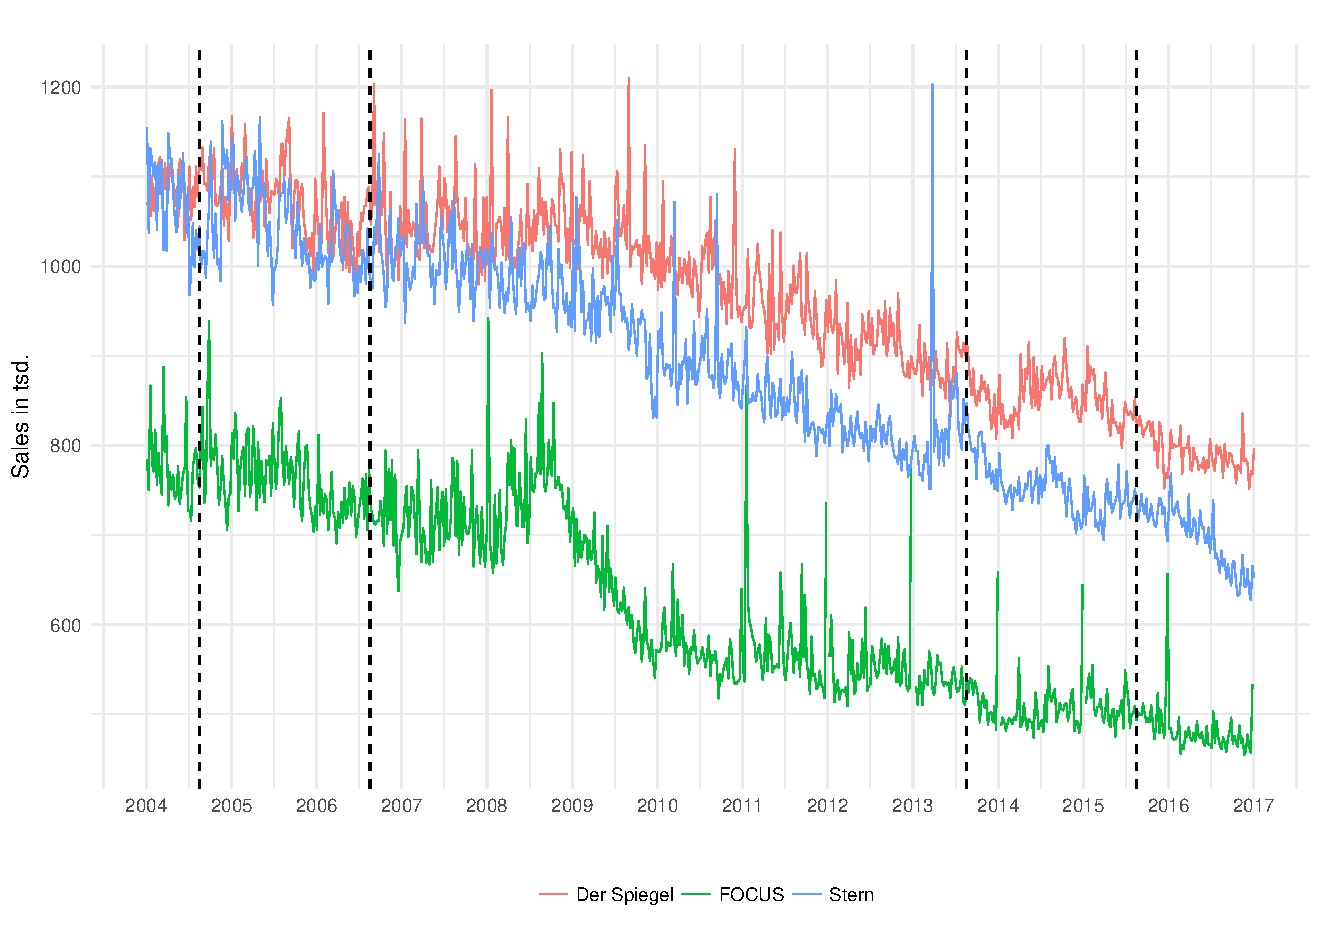
\includegraphics[scale=0.5]{circ_fss.eps}
\end{minipage}
\hfill
\begin{minipage}[hbt]{7cm}
	\centering
	\includegraphics[scale=0.5]{circ_fss2.eps}
\end{minipage}
\label{fig:fss}
\end{figure}

\begin{figure}[H]
\caption{Adjusted Sales (ARIMA)}
\begin{minipage}[hbt]{7cm}
	\centering
	\includegraphics[scale=0.5]{circ_arma_fss.eps}
\end{minipage}
\hfill
\begin{minipage}[hbt]{7cm}
	\centering
	\includegraphics[scale=0.5]{circ_arma_fss2.eps}
\end{minipage}
\label{fig:fss_arima}
\end{figure}

\begin{figure}[H]
\caption{Adjusted Sales (OLS)}
\begin{minipage}[hbt]{7cm}
	\centering
	\includegraphics[scale=0.5]{circ_ols_fss.eps}
\end{minipage}
\hfill
\begin{minipage}[hbt]{7cm}
	\centering
	\includegraphics[scale=0.5]{circ_ols_fss2.eps}
\end{minipage}
\label{fig:fss_ols}
\end{figure}

\begin{table}[htbp]
  \centering
  \caption{Cross-correlation functions news nagazines (reader market)}
       \begin{tabular}{crrr|rrrr}
    \textcolor[rgb]{ 1,  1,  1}{} & \textcolor[rgb]{ 1,  1,  1}{} & \textcolor[rgb]{ 1,  1,  1}{} & \multicolumn{1}{c}{\textcolor[rgb]{ 1,  1,  1}{}} & \textcolor[rgb]{ 1,  1,  1}{} & \textcolor[rgb]{ 1,  1,  1}{} & \textcolor[rgb]{ 1,  1,  1}{} & \textcolor[rgb]{ 1,  1,  1}{} \\
    \midrule
    \midrule
          & \multicolumn{1}{c}{Focus} & \multicolumn{1}{c}{Focus} & \multicolumn{1}{c}{Stern} & \multicolumn{1}{c}{Focus} & \multicolumn{1}{c}{Focus} & \multicolumn{1}{c}{Stern} & \multicolumn{1}{c}{\textit{SE_-^+}} \\
          & \multicolumn{1}{c}{Der Spiegel} & \multicolumn{1}{c}{Stern} & \multicolumn{1}{c}{Der Spiegel} & \multicolumn{1}{c}{Der Spiegel} & \multicolumn{1}{c}{Stern} & \multicolumn{1}{c}{Der Spiegel} &  \\
    \midrule
          & \multicolumn{6}{c}{\textbf{2004 - 2006}}      & \multicolumn{1}{c}{$\pm$.20} \\
    \midrule
    t     & \multicolumn{3}{c|}{\textbf{ARIMA}} & \multicolumn{3}{c}{\textbf{OLS}} &  \\
    -6    & 0.211 & 0.057 & 0.057 & 0.144 & 0.096 & 0.128 &  \\
    -5    & 0.042 & -0.057 & 0.087 & 0.062 & 0.030 & 0.120 &  \\
    -4    & -0.015 & -0.115 & -0.084 & 0.008 & -0.022 & 0.037 &  \\
    -3    & 0.006 & \textbf{-0.212} & -0.010 & 0.104 & -0.155 & 0.099 &  \\
    -2    & 0.169 & -0.083 & 0.100 & 0.273 & -0.155 & 0.145 &  \\
    -1    & 0.049 & 0.060 & \textbf{0.272} & 0.154 & -0.035 & 0.160 &  \\
    0     & \textbf{-0.300} & -0.041 & -0.190 & \textbf{-0.265} & -0.096 & \textbf{-0.493} &  \\
    1     & 0.025 & 0.172 & 0.076 & -0.001 & 0.135 & 0.121 &  \\
    2     & 0.094 & -0.145 & 0.127 & 0.195 & -0.155 & 0.171 &  \\
    3     & 0.094 & -0.030 & 0.138 & 0.165 & -0.127 & 0.184 &  \\
    4     & -0.074 & 0.124 & 0.155 & -0.042 & 0.034 & 0.170 &  \\
    5     & 0.087 & 0.123 & -0.053 & 0.095 & 0.055 & 0.052 &  \\
    6     & 0.118 & -0.026 & -0.084 & 0.227 & -0.070 & -0.003 &  \\
    \midrule
    \multicolumn{1}{|r}{} & \multicolumn{6}{c}{\textbf{2014 - 2016}}      & \multicolumn{1}{c}{$\pm$.21} \\
    \midrule
          & \multicolumn{3}{c|}{\textbf{ARIMA}} & \multicolumn{3}{c}{\textbf{OLS}} &  \\
    -6    & -0.103 & -0.060 & -0.090 & -0.143 & -0.010 & -0.004 &  \\
    -5    & \textbf{0.226} & 0.072 & -0.115 & 0.096 & 0.071 & -0.057 &  \\
    -4    & 0.053 & 0.047 & 0.046 & 0.055 & 0.053 & 0.042 &  \\
    -3    & -0.010 & 0.008 & 0.017 & -0.005 & 0.049 & 0.059 &  \\
    -2    & \textbf{-0.293} & 0.086 & 0.032 & \textbf{-0.242} & 0.171 & 0.091 &  \\
    -1    & 0.136 & -0.048 & 0.077 & 0.019 & -0.025 & 0.027 &  \\
    0     & -0.027 & -0.098 & \textbf{-0.286} & -0.110 & -0.118 & \textbf{-0.479} &  \\
    1     & 0.065 & 0.216 & 0.078 & -0.030 & 0.209 & 0.021 &  \\
    2     & \textbf{0.222} & 0.070 & 0.124 & 0.178 & 0.067 & 0.121 &  \\
    3     & 0.195 & -0.009 & 0.030 & 0.231 & -0.020 & 0.090 &  \\
    4     & -0.023 & -0.028 & 0.108 & 0.092 & -0.012 & 0.153 &  \\
    5     & -0.002 & -0.049 & 0.014 & 0.087 & -0.022 & 0.102 &  \\
    6     & 0.057 & -0.048 & 0.151 & 0.078 & -0.058 & 0.185 &  \\
    \bottomrule
    \bottomrule
    \end{tabular}%
  \label{tab:ccf_fss}%
\end{table}%

\begin{figure}[H]
\caption{News Magazines total ad pages}
\begin{minipage}[hbt]{7cm}
	\centering
	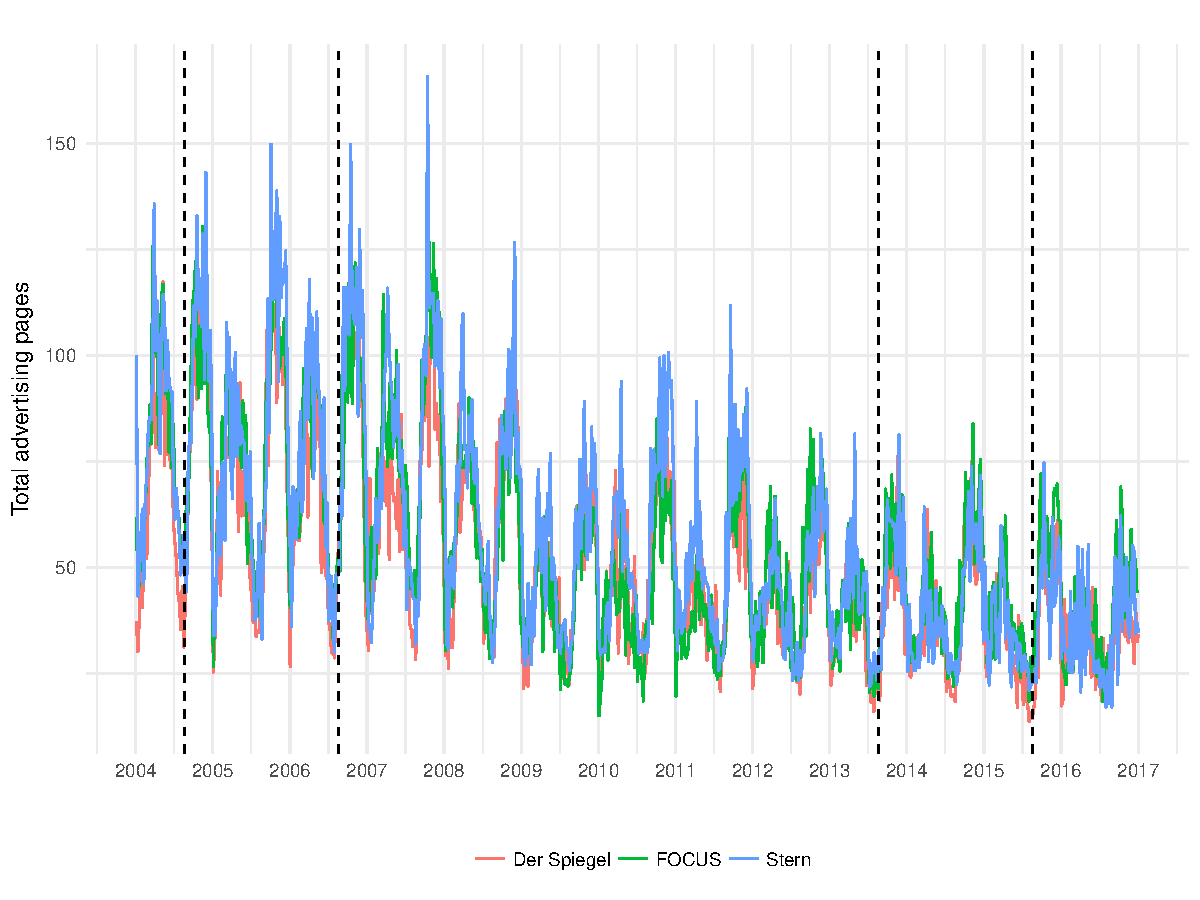
\includegraphics[scale=0.5]{ads_fss.eps}
\end{minipage}
\hfill
\begin{minipage}[hbt]{7cm}
	\centering
	\includegraphics[scale=0.5]{ads_fss2.eps}
\end{minipage}
\label{fig:fss2}
\end{figure}

\begin{figure}[H]
\caption{Adjusted ad pages (ARIMA)}
\begin{minipage}[hbt]{7cm}
	\centering
	\includegraphics[scale=0.5]{ads_arma_fss.eps}
\end{minipage}
\hfill
\begin{minipage}[hbt]{7cm}
	\centering
	\includegraphics[scale=0.5]{ads_arma_fss2.eps}
\end{minipage}
\label{fig:fss_arima2}
\end{figure}

\begin{figure}[H]
\caption{Adjusted ad pages (OLS)}
\begin{minipage}[hbt]{7cm}
	\centering
	\includegraphics[scale=0.5]{ads_ols_fss.eps}
\end{minipage}
\hfill
\begin{minipage}[hbt]{7cm}
	\centering
	\includegraphics[scale=0.5]{ads_ols_fss2.eps}
\end{minipage}
\label{fig:fss_ols2}
\end{figure}

\begin{table}[htbp]
  \centering
  \caption{Cross-correlation functions news magazines (advertising market)}
    \begin{tabular}{crrr|rrrr}
    \toprule
    \toprule
          & \multicolumn{1}{c}{Focus} & \multicolumn{1}{c}{Focus} & \multicolumn{1}{c}{Stern} & \multicolumn{1}{c}{Focus} & \multicolumn{1}{c}{Focus} & \multicolumn{1}{c}{Stern} & \multicolumn{1}{c}{\textit{SE_-^+}} \\
          & \multicolumn{1}{c}{Der Spiegel} & \multicolumn{1}{c}{Stern} & \multicolumn{1}{c}{Der Spiegel} & \multicolumn{1}{c}{Der Spiegel} & \multicolumn{1}{c}{Stern} & \multicolumn{1}{c}{Der Spiegel} &  \\
    \midrule
    Lags  & \multicolumn{6}{c}{\textbf{2004 - 2006}}      & \multicolumn{1}{c}{$\pm$.20} \\
    \midrule
          & \multicolumn{3}{c|}{\textbf{ARIMA}} & \multicolumn{3}{c}{\textbf{OLS}} &  \\
    -6    & -0.038 & 0.039 & 0.051 & -0.051 & 0.048 & -0.061 &  \\
    -5    & 0.016 & -0.021 & 0.053 & -0.040 & -0.099 & 0.179 &  \\
    -4    & -0.002 & -0.147 & 0.116 & -0.096 & -0.164 & -0.009 &  \\
    -3    & -0.015 & -0.067 & 0.093 & 0.039 & -0.012 & 0.114 &  \\
    -2    & -0.053 & 0.047 & 0.028 & -0.088 & 0.026 & -0.061 &  \\
    -1    & 0.035 & -0.026 & 0.143 & -0.004 & -0.073 & 0.184 &  \\
    0     & \textbf{-0.604} & \textbf{-0.288} & \textbf{-0.415} & \textbf{-0.647} & \textbf{-0.310} & \textbf{-0.417} &  \\
    1     & -0.050 & 0.016 & 0.074 & -0.015 & 0.030 & 0.177 &  \\
    2     & 0.072 & 0.096 & -0.014 & -0.040 & 0.068 & -0.153 &  \\
    3     & 0.068 & 0.095 & -0.039 & 0.051 & 0.052 & 0.042 &  \\
    4     & -0.006 & 0.037 & 0.079 & -0.074 & -0.026 & -0.034 &  \\
    5     & -0.037 & -0.051 & 0.050 & 0.029 & 0.024 & 0.134 &  \\
    6     & 0.156 & 0.034 & -0.139 & 0.141 & 0.032 & \textbf{-0.213} &  \\
    \midrule
    \multicolumn{1}{|r}{} & \multicolumn{6}{c}{\textbf{2014 - 2016}}      & \multicolumn{1}{c}{$\pm$.20} \\
    \midrule
    t     & \multicolumn{3}{c|}{\textbf{ARIMA}} & \multicolumn{3}{c}{\textbf{OLS}} &  \\
    -6    & -0.110 & 0.098 & 0.087 & -0.012 & 0.121 & 0.050 &  \\
    -5    & -0.015 & 0.134 & -0.057 & 0.145 & 0.018 & -0.086 &  \\
    -4    & 0.100 & -0.088 & 0.164 & 0.077 & -0.109 & 0.138 &  \\
    -3    & 0.142 & -0.019 & 0.043 & 0.054 & 0.026 & 0.024 &  \\
    -2    & 0.210 & -0.038 & -0.087 & 0.020 & -0.023 & -0.108 &  \\
    -1    & 0.238 & 0.179 & -0.052 & -0.086 & 0.155 & 0.051 &  \\
    0     & \textbf{-0.398} & \textbf{-0.246} & \textbf{-0.324} & \textbf{-0.545} & \textbf{-0.352} & \textbf{-0.398} &  \\
    1     & 0.038 & 0.032 & 0.065 & -0.157 & 0.161 & 0.033 &  \\
    2     & -0.063 & 0.190 & 0.157 & \textbf{-0.258} & 0.182 & 0.043 &  \\
    3     & 0.011 & 0.241 & -0.110 & -0.013 & 0.012 & -0.088 &  \\
    4     & -0.127 & -0.041 & 0.164 & -0.080 & -0.070 & 0.178 &  \\
    5     & 0.032 & 0.077 & -0.074 & 0.065 & 0.039 & -0.016 &  \\
    6     & 0.078 & -0.008 & 0.029 & 0.082 & 0.007 & -0.018 &  \\
    \bottomrule
    \bottomrule
    \end{tabular}%
  \label{tab:ccf_fss2}%
\end{table}%

\bibliography{Meine Bibliothek}

\end{document}
